\documentclass[a4paper,11pt,notitlepage]{report}

\usepackage{graphicx}
\usepackage[utf8]{inputenc}
\usepackage[T1]{fontenc}
\usepackage[ngerman]{babel}
\usepackage{bibgerm}
\usepackage{amsmath,amssymb,amsthm}
\usepackage{color}
\usepackage{enumerate}
\usepackage{tabularx}
\usepackage{subfig}
\usepackage{fancyhdr}
\usepackage{upgreek}
\usepackage[pdftex,pdfpagelabels,colorlinks,backref,pagebackref]{hyperref}
\usepackage{tikz} % SELBST HINZUGEFÜGT
\usepackage{graphicx}
\usepackage{framed}
\usepackage{lmodern}
% == Set the heading style ===================================================
\setlength{\headheight}{14pt}
\pagestyle{fancyplain}
\renewcommand{\chaptermark}[1]{\markboth{#1}{}}
\renewcommand{\sectionmark}[1]{\markright{\thesection\ #1}}
\lhead[\fancyplain{}{\thepage}]{\fancyplain{}{\rightmark}}
\rhead[\fancyplain{}{\leftmark}]{\fancyplain{}{\thepage}}
\cfoot{}
\renewcommand{\headrulewidth}{0.4pt}
% ============================================================================

% == Set correct values for fitting floats ===================================
\tolerance=2000
\emergencystretch=10pt

\setcounter{topnumber}{3}
\setcounter{totalnumber}{5}
\setcounter{bottomnumber}{2}

% To make those darn floats fit where they should
\setcounter{totalnumber}{9}
\setcounter{topnumber}{9}
\setcounter{bottomnumber}{9}
\renewcommand{\textfraction}{0.00}
\renewcommand{\topfraction}{1.0}
\renewcommand{\bottomfraction}{1.0}
% ============================================================================

% == German definitions for theorems etc. ==================================== 
\newtheorem{definition}{Definition}[chapter]
\newtheorem{theorem}{Satz}[chapter]
\newtheorem{lemma}{Lemma}[chapter]
\newtheorem{proposition}{Proposition}[chapter]
\newtheorem{corollary}{Korollar}[chapter]
\newtheorem{observation}{Beobachtung}[chapter]
\newtheorem{fact}{Fakt}[chapter]
\newtheorem{remark}{Bemerkung}[chapter]
\newtheorem{example}{Beispiel}[chapter]
% ============================================================================

% == Abkürzungen für die reellen, natürlichen, ganzen,... Zahlen =============
\newcommand{\R}{{\ensuremath{\mathbb{R}}}}
\newcommand{\N}{{\ensuremath{\mathbb{N}}}}
\newcommand{\Z}{{\ensuremath{\mathbb{Z}}}}
\newcommand{\C}{{\ensuremath{\mathbb{C}}}}
\newcommand{\Q}{{\ensuremath{\mathbb{Q}}}}
\newcommand{\F}{{\ensuremath{\mathbb{F}}}}
\newcommand{\Prim}{{\ensuremath{\mathbb{P}}}}
% ============================================================================

% == Makros für Autorenname und -adresse =====================================
\newcommand{\myaddress}[6]{%
  \parbox{\textwidth}{\textbf{\large #1}\\
    #2\\ #3\\ #4\\ 
    \ifthenelse{\equal{#5}{}}{}{Email: \href{mailto:#5}{\texttt{#5}}\\}
    \ifthenelse{\equal{#6}{}}{}{WWW: \href{#6}{\path|#6|}\\}
  } 
}

\newcommand{\myauthor}[1]{%
  \addtocontents{toc}{\protect\hspace{3.35ex}%
  \textsl{#1}\par}\vspace{-4ex}\quad\hfill\textsl{\Large #1}\vspace{8ex}}

\newcommand{\myname}[1]{\Large #1}

%%%%%%%%%%%%%%%%%%%%%%%%%%%%%%%%%%%%%%%%%%%%%%%%%%
% Tragen Sie in der folg. Zeile Ihren Namen ein: %
%%%%%%%%%%%%%%%%%%%%%%%%%%%%%%%%%%%%%%%%%%%%%%%%%%

\newcommand{\OO}{{\ensuremath{\mathcal{O}}}}

\renewcommand{\thechapter}{\Roman{chapter}}
\renewcommand{\thesection}{\arabic{section}}


\newenvironment{Kasten}[1]
{
\hspace{0.05\linewidth}
\begin{center}
\begin{minipage}{0.9\linewidth}
\setlength{\fboxsep}{10pt}
%\setlength{\fboxsep}{18pt}
%\definecolor{shadecolor}{gray}{0.9}
\definecolor{shadecolor}{gray}{1}
\definecolor{framecolor}{gray}{0}
\def\FrameCommand{\fcolorbox{framecolor}{shadecolor}}
\MakeFramed {\FrameRestore}
\subsection{#1}
\begin{itshape}
}
{
\end{itshape}
\endMakeFramed
\end{minipage}
\end{center}
%\vspace{1em}
}

\begin{document}
\shorthandoff{"}
\setcounter{chapter}{0}

\begin{titlepage}
	\begin{center}	
		\LARGE \textbf{{Einführung in die Geometrie und Topologie - Definitionen -} \\[5ex] 
    		{\Large Vorlesung im Wintersemester 2011/2012\\[5ex]}}
	\end{center}
	\begin{center}
		\Large Sarah Lutteropp, Simon Bischof
	\end{center}
	\begin{center}
		\today
	\end{center}
	\vspace{2cm}
	\begin{center}
		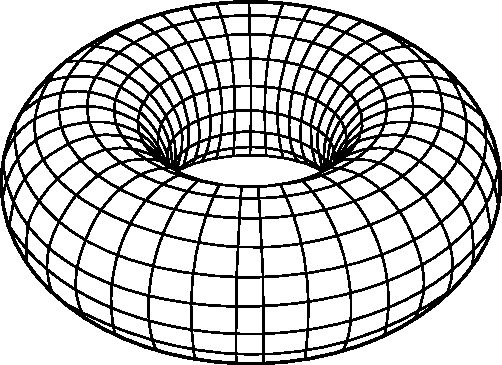
\includegraphics[width=0.8\textwidth]{torus2.pdf}
	\end{center}
\end{titlepage}
%\maketitle
\setcounter{tocdepth}{1}
\tableofcontents

\section{Topologischer Raum}
Ein \underline{topologischer Raum} $X$ ist gegeben durch eine Menge $X$ und ein System $\OO$ von Teilmengen von $X$, den so genannten \underline{offenen Mengen} von $X$, welches unter beliebigen Vereinigungen und endlichen Durchschnitten abgeschlossen ist und $X$ und die leere Menge $\emptyset$ als Elemente enthält.
\newline
$X$ Menge, $\OO \subset \mathcal{P}(X) \colon$
\begin{enumerate}[(1)]
	\item $O_1, O_2 \in \OO \Rightarrow O_1 \cap O_2 \in \OO$
	\item $O_\alpha \in \OO, \alpha \in A, A \text{ Indexmenge} \Rightarrow \bigcup\limits_{\alpha \in A}{O_\alpha} \in \OO$
	\item $X, \emptyset \in \OO$
\end{enumerate}


\section{Metrischer Raum}
Ein \underline{metrischer Raum} $X$ ist eine Menge $X$ mit einer Abbildung $d \colon X \times X \rightarrow \R$, der \underline{"Metrik"} auf $X$, die folgende Eigenschaften erfüllt:
$\forall x,y,z \in X$
\begin{enumerate}[(1)]
	\item $d(x,y) = d(y,x)$ \underline{"Symmetrie"}
	\item $d(x,y) = 0 \Leftrightarrow x = y, d(x,y) \geq 0$ \underline{"Definitheit"}
	\item $d(x,z) \leq d(x,y) + d(y,z)$ \underline{"Dreiecksungleichung"}
\end{enumerate}


\section{Stetigkeit}
Eine Abbildung $F \colon X \rightarrow Y$ zwischen topologischen Räumen $X$ und $Y$ heißt \underline{stetig}, falls die F-Urbilder offener Mengen in $Y$ offene Teilmengen von $X$ sind.


\section{Homotopie}
Eine \underline{Homotopie} $H \colon f \simeq g$ zwischen zwei (stetigen) Abbildungen $f,g \colon X \rightarrow Y$ ist eine (stetige) Abbildung $$H \colon X \times I \footnote{$I = [0,1] \subset \R$} \rightarrow Y, (x,t) \mapsto H(x,t)$$ mit $H(x,0) = f(x) \text{ und } H(x,1) = g(x) \forall x \in X$.


\section{Homotope Abbildungen}
	Zwei (stetige) Abbildungen heißen \underline{homotop}, in Zeichen: $f \simeq g$, falls eine Homotopie mit Anfang $f$ und Ende $g$ existiert.


\section{Nullhomotopie}
Eine stetige Abbildung $f \colon X \rightarrow Y$ heißt \underline{nullhomotop}, falls sie homotop zu einer konstanten Abbildung ist.


\section{Teilraumtopologie}
Es sei $(X, \OO)$ topologischer Raum und $A \subset X$. Die auf $A$ durch
$$\OO \Big |_{A} := \{U \cap A \mid U \in \OO \}$$
induzierte Topologie heißt \underline{Teilraumtopologie} und der dadurch gegebene topologische Raum $(A, \OO \Big |_{A})$ heißt \underline{Teilraum} von $(X, \OO)$.


\section{Abgeschlossenheit}
	$A \subset X, X$ topologischer Raum, heißt \underline{abgeschlossen} $:\Leftrightarrow X \backslash A \text{ ist offen}$.


\section{Umgebung}
	Ist $X$ topologischer Raum und $x \in X$, so heißt jede \underline{offene} Teilmenge $O \subset X$ mit $x \in O$ eine \underline{Umgebung} von $x$.


\section{Basis}
	Ist $(X, \OO)$ topologischer Raum mit $\mathcal{B} \subset \OO$, so heißt $\mathcal{B}$ \underline{Basis der Topologie} $:\Leftrightarrow$ Jede (nichtleere) offene Menge ist Vereinigung von Mengen aus $\mathcal{B}$.



\section{Feiner und gröber}
	Sind $\OO_1$ und $\OO_2$ Topologien auf $X$ und $\OO_1 \subset \OO_2$, so heißt $\OO_2$ \underline{feiner} als $\OO_1$ und $\OO_1$ \underline{gröber} als $\OO_2$.


\section{$\epsilon$-Ball, Sphäre}
	Für einen metrischen Raum $(X,d)$ und $\epsilon > 0$ sei für $p \in X$
	\begin{itemize}
		\item $B_\epsilon(p):=\{x \in C \mid d(p,x) < \epsilon \}$ der \underline{offene $\epsilon$-Ball um $p$}
		\item $D_\epsilon(p):=\{x \in C \mid d(p,x) \leq \epsilon \}$ der \underline{abgeschlossene $\epsilon$-Ball um $p$}
		\item $S_\epsilon(p):=\{x \in C \mid d(p,x) = \epsilon \}$ die \underline{ $\epsilon$-Sphäre} um $p$ (oder \underline{Sphäre vom Radius $\epsilon$})
	\end{itemize}


\section{Metrischer Unterraum}
	Ist $(X,d)$ metrischer Raum und $A \subset X$, so heißt der metrische Raum $(A, d \big |_{A \times A})$ \underline{(metrischer) Unterraum von $X$}.


\section{Beschränktheit, Durchmesser}
	$A \subset (X,d)$ heißt \underline{beschränkt} \newline $:\Leftrightarrow \exists 0 < \rho \in \R \colon d(x,y) < \rho  \text{   } \forall x,y \in A$
	\newline
	Das Infimum, diam $A$, dieser $\rho$ heißt dann \underline{Durchmesser von $A$}.
	\newline


\section{Abstand}
	$(X,d)$ sei metrischer Raum und $A \subset X, p \in X$.
	$$d(p,A) := dist(p,A):= \inf \{d(p,a) \mid a\in A \}$$
	heißt \underline{Abstand von $p$ und $A$}.


\section{Innerer Punkt, äußerer Punkt, Randpunkt}
	Für $p \in A \subset X$, $X$ topologischer Raum, heißt $p$
	\newline
	\begin{enumerate}[(1)]
		\item \underline{innerer Punkt} von $A$, falls es eine in $A$ enthaltene Umgebung $U$ um $p$ gibt. 
		\item \underline{äußerer Punkt}, falls eine zu $p$ disjunkte Umgebung $V$ in $X$ existiert.
		\item \underline{Randpunkt von $A$}, falls jede Umgebung von $p$ nichtleeren Durchschnitt mit $A$ und $X \backslash A$ hat.
	\end{enumerate}


\section{Inneres}
	Für $A \subset X$ heißt die größte in $X$ offene und in $A$ enthaltene Teilmenge $\mathring A$ \underline{Inneres von $A$}.


\section{Abschluss}
	Der \underline{Abschluss} $\bar{A}$ von $A$ ist $X \backslash \left ( \mathring {(X \backslash A} ) \right )$.


\section{Rand}
	Der \underline{Rand} $\partial A$ von $A$ ist $\partial A := \bar{A} \backslash \mathring A$, d.h. Rand $A$ = \{ Randpunkte von A \}.


\section{Stetigkeit}
	$f \colon X \rightarrow Y$ ist stetig $:\Leftrightarrow \forall$ offenen Mengen in $Y$ ist das Urbild unter $f$ offene Menge in $X$.


\section{Stetigkeit} %spacings stimmen nicht ganz (TODO)
	$f \colon X \rightarrow Y$ ist stetig in $x \in X$
	$:\Leftrightarrow \forall \text{ Umgebungen } V \text{ von } f(x) \exists \text{ Umgebung } U \text{ von } x \text{ mit } f(U) \subset V$.
	\newline


\section{Isometrische Einbettung, Isometrie}
	Sind $X,Y$ metrische Räume, so heißt eine Abbildung $f \colon X \rightarrow Y$ \underline{isometrische Einbettung}
	\newline	
	 $: \Leftrightarrow \forall x, x^\prime \in X$ gilt $d_Y \left ( f(x), f(x^\prime) \right ) = d_X (x, x^\prime)$.
	\newline
	Eine isometrische Einbettung ist immer injektiv.
	\newline
	Ist $f$ zusätzlich \underline{bijektiv}, so heißt $f$ \underline{\underline{Isometrie}}. 


\section{Homöomorphismus}
	Eine invertierbare Abbildung $f \colon X \rightarrow Y$ topologischer Räume heißt \underline{Homöomorphismus}, falls $f$ und $f^{-1}$ stetig sind.


\section{homöomorph}
	Zwei topologische Räume $X$ und $Y$ heißen \underline{homöomorph} oder \underline{vom gleichen Homöomorphietyp}, in Zeichen $X \cong Y$, falls es einen Homöomorphismus $f \colon X \rightarrow Y$ gibt.


\section{Einbettung}
	$f \colon X \rightarrow Y$ stetig heißt \underline{Einbettung} $:\Leftrightarrow X \overset{f}{\rightarrow}f(X) \subset Y$ Homöomorphismus.


\section{Äquivalenz von Einbettungen}
	Zwei Einbettungen $f,g \colon X \rightarrow Y$ heißen \underline{äquivalent} $:\Leftrightarrow \exists \text{ Homöomorphismen } h_X \colon X \rightarrow X, h_Y \colon Y \rightarrow Y \text{ mit } g \circ h_X = h_Y \circ f$, d.h. dass das Diagramm 
		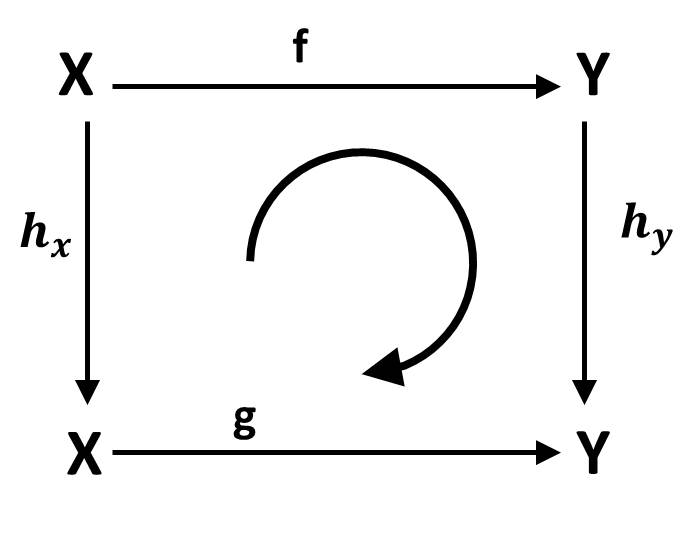
\includegraphics[scale=0.3]{images/homotopieaequivalenz.jpg} kommutiert.


\section{Knoten}
	Eine Einbettung $S^1 \rightarrow \R^3$ heißt \underline{Knoten}.


\section{zusammenhängend}
	Ein topologischer Raum heißt \underline{zusammenhängend} $:\Leftrightarrow$ Die einzigen in $X$ gleichzeitig offenen und abgeschlossenen Teilmengen sind $\emptyset$ und $X$.
	\newline
	Ansonsten heißt $X$ \underline{un-} oder \underline{nicht zusammenhängend}.


\section{Überdeckung}
	Eine Familie $\mathcal{U} = \{U_\alpha \mid \alpha \in A\}$\footnote{$A$ Indexmenge} von Teilmengen von $X$ heißt \underline{Überdeckung von $X$} $:\Leftrightarrow X = \bigcup\limits_{\alpha \in A}{U_\alpha}$.
	\newline
	$\mathcal{U}$ heißt \underline{offene} beziehungsweise \underline{abgeschlossene} Überdeckung $\Leftrightarrow$ alle $U_\alpha$ sind offen beziehungsweise abgeschlossen.
	\newline
	Für $X^\prime \subset X$ heißt eine Familie $\mathcal{U} = \{U_\alpha\}$ wie oben Überdeckung von $X^\prime$ $:\Leftrightarrow X^\prime \subset \bigcup\limits_{\alpha \in A}{U_\alpha}$.
	\newline


\section{Partition}
	Eine \underline{Partition} oder \underline{Zerlegung} einer Menge ist eine Überdeckung dieser Menge durch paarweise disjunkte Teilmengen.
	\newline


\section{Zusammenhangskomponente}
	Eine \underline{Zusammenhangskomponente} eines topologischen Raumes $X$ ist eine maximale zusammenhängende Teilmenge von $X$.


\section{Weg, Anfangspunkt, Endpunkt}
	ein \underline{Weg} in einem topologischen Raum $X$ ist eine stetige Abbildung $\gamma \colon [0,1] \rightarrow X$, und $\gamma(0)$ heißt \underline{Anfangs-}, $\gamma(1)$ \underline{Endpunkt}.
	\newline


\section{Wegzusammenhang}
	$X$ heißt \underline{wegzusammenhängend} $:\Leftrightarrow$ Zu je zwei Punkten $x,x^\prime \in X \exists \text{ Weg } \gamma \colon [0,1] \rightarrow X \text{ mit } \gamma(0)=x, \gamma(1)=x^\prime$.
	\newline


\section{Kompaktheit}
	Ein topologischer Raum $X$ heißt \underline{kompakt}, falls jede offene Überdeckung von $X$ eine endliche Teilüberdeckung enthält.


\section{$T_1$-Raum}
Ein topologischer Raum $X$ heißt \underline{$T_1$-Raum} bzw. \underline{erfüllt das erste Trennungsaxiom} $:\Leftrightarrow$ Für je zwei verschiedene Punkte von $X$ existiert für jeden dieser Punkte eine Umgebung in $X$, die den anderen nicht enthält.
\newline
$\forall x \neq y \in X \exists U = U_X \colon y \notin U_X$ 


\section{$T_2$-Raum}
	$X$ heißt \underline{Hausdorff}- oder \underline{$T_2$-Raum} bzw. \underline{erfüllt das zweite Trennungsaxiom} $:\Leftrightarrow$ Je zwei verschiedene Punkte in $X$ besitzen disjunkte Umgebungen.
	\newline
	$\forall x \neq y \in X \exists U_x \ni x, U_y \ni y$ mit $U_x \cap U_y = \emptyset$


\section{Grenzwert}
Ist $(x_n)_{n \in \N}$ eine Folge von Punkten in einem topologischen Raum $X$, so heißt $x \in X$ \underline{Grenzwert} der Folge $(x_n)$ genau dann, wenn zu jeder Umgebung $U$ von $x$ ein $N \in \N$ existiert mit $x_n \in U \forall n \geq N$. 
\newline


\section{Umgebungsbasis}
	Ist $X$ topologischer Raum und $x \in X$, so ist eine \underline{Umgebungsbasis} oder \underline{Basis von $X$} \underline{\underline{in $x$}} eine Familie von Umgebungen von $x$, sodass \underline{jede} Umgebung von $x$ eine Umgebung aus der Familie enthält.


\section{Abzählbarkeitsaxiome, Separabilität}
	$X$ \underline{erfüllt das erste Abzählbarkeitsaxiom}
	$:\Leftrightarrow$ jeder Punkt $x \in X$ besitzt eine abzählbare Basis.
	\newline
	$X$ \underline{erfüllt das zweite Abzählbarkeitsaxiom}
	$:\Leftrightarrow$ $X$ selbst besitzt eine abzählbare Basis.
	\newline
	$X$ heißt \underline{separabel} $:\Leftrightarrow$ $X$ enthält eine abzählbare und dichte ($\bar{A} = X$) Menge $A$.

 
\section{Lokale Kompaktheit}
$X$ heißt \underline{\underline{lokal} kompakt} \newline $:\Leftrightarrow$ Jeder Punkt $x \in X$ besitzt eine Umgebung $U$, sodass $\overline{U}$ kompakt ist.
 

\section{Lokale Endlichkeit}
	Eine Familie $\Gamma$ von Teilmengen eines topologischen Raumes $X$ heißt \underline{lokal endlich} $:\Leftrightarrow \forall x \in X \exists U = U(x) \colon A \cap U = \emptyset \forall A \in \Gamma$ bis auf endlich viele $A$.

 
\section{Verfeinerung}
	$\Gamma, \Delta$ Überdeckungen von $X$. $\Delta$ heißt \underline{Verfeinerung} von $\Gamma$ \newline $:\Leftrightarrow \forall A \in \Delta \exists B \in \Gamma \colon A \subset B$.
 

\section{Parakompaktheit}
	$X$ heißt \underline{parakompakt} $:\Leftrightarrow$ Jede offene Überdeckung besitzt eine lokal endliche offene Verfeinerung. 


\section{Mannigfaltigkeit, Karte}
	Ein topologischer Raum $M$ heißt \underline{$n$-dimensionale} \underline{(topologische) Mannigfaltigkeit}, wenn gilt:
	\begin{enumerate}
		\item $M$ ist ein Hausdorff-Raum mit abzählbarer Basis der Topologie
		\item $M$ ist lokal homöomorph zu $\R^n$, d.h. zu jedem $p \in M$ existieren eine Umgebung $U=U(p) \subset_{offen} M$ und ein Homöomorphismus $\varphi \colon U \rightarrow V, V \subset_{offen} \R^n$.
			\newline
			Jedes solche Paar $(U,\varphi)$ heißt eine \underline{Karte} oder ein \underline{lokales Koordinatensystem} um $p$.
	\end{enumerate}


\section{Atlas}
	Ein \underline{Atlas} für eine topologische $n$-Mannigfaltigkeit $M$ ist eine Menge $\mathcal{A} = \{(\varphi_\alpha, U_\alpha) \mid \alpha \in \Lambda\}$\footnote{$\Lambda$ Indexmenge}
	von Karten $\varphi_\alpha \colon U_\alpha \rightarrow V_\alpha = \varphi(U_\alpha) \subset \R^n$, so dass $M = \bigcup\limits_{a \in \Lambda}{U_\alpha}$


\section{$C^k$-Atlas, Kartenwechsel}
	Ein Atlas heißt \underline{differenzierbar} \underline{von der Klasse $C^k$} (oder: $C^k$-Atlas von $M$), wenn für alle $\alpha, \beta \in \Lambda$ mit $U_\alpha \cap U_\beta \neq \emptyset$ der \underline{Kartenwechsel} $\varphi_\beta \circ \varphi_\alpha^{-1} \colon \varphi_\alpha(U_\alpha \cap U_\beta) \rightarrow \varphi_\beta(U_\alpha \cap U_\beta)$ eine $C^k$-Abbildung, also $k$-mal stetig differenzierbar ist. $(k=0,1,2,\ldots,\infty,\omega)$
	\newline

 
\section{Verträglichkeit, differenzierbare Struktur}
	Ist $M$ topologische Mannigfaltigkeit und $\mathcal{A}=\{(\varphi_\alpha,U_\alpha) \mid \alpha \in \Lambda\}$ ein $C^k$-Atlas von $M$, so heißt eine Karte $(\varphi,U)$ von $M$ \underline{mit $\mathcal{A}$ verträglich}, falls $\mathcal{A}^\prime := \mathcal{A} \cup \{(\varphi,U)\}$ ebenfalls $C^k$-Atlas ist. 
	Ein $C^k$-Atlas heißt \underline{maximal} (oder \underline{differenzierbare Struktur} (der Klasse $C^k$)), falls $\mathcal{A}$ alle mit $\mathcal{A}$ verträglichen Karten enthält.
 

\section{$C^k$-Mannigfaltigkeit, glatt}
	Eine \underline{differenzierbare Mannigfaltigkeit der Klasse $C^k$} (kurz: $C^k$-Mannigfaltigkeit) ist ein Paar $(M,\mathcal{A})$ bestehend aus einer topologischen Mannigfaltigkeit $M$ und einer $C^k$-Struktur auf $M$. Eine $C^\infty$-Mannigfaltigkeit heißt auch \underline{\underline{glatt}}.
	\newline


\section{Produkt-Topologie}
	Sind $(X, \OO_X)$ und $(Y, \OO_Y)$ topologische Räume, so bildet $$\mathcal{B}_{X \times Y} := \{U \times V \mid U \in \OO_X, V \in \OO_Y\}$$
	die Basis einer Topologie für die Menge $X \times Y$, und diese heißt \underline{Produkt-Topologie auf $X \times Y$}.
	\newline
	Versehen mit der Produkt-Topologie ist $X \times Y$ sebst ein topologischer Raum und für gegebene $X, Y$ denkt man sich $X \times Y$ stillschweigend mit der Produkt-Topologie versehen.


\section{$C^l$-Abbildung}
Es seien $(M, \mathcal{A})$ eine $n$-dimensionale $C^k$-Mannigfaltigkeit, $(M^\prime, \mathcal{A}^\prime)$ eine $n^\prime$-dimensionale $C^{k^\prime}$-Mannigfaltigkeit und $l \leq \min(k,k^\prime)$. Eine stetige Abbildung $f \colon M \rightarrow M^\prime$ heißt \underline{differenzierbar} (\underline{von der Klasse $C^l$}) oder kurz: $C^l$-Abbildung, falls gilt:
$$\forall (\varphi,U) \in \mathcal{A} \text{ und } (\varphi^\prime, U^\prime) \in \mathcal{A}^\prime \text{ mit } f(U) \cap U^\prime \neq \emptyset \text{ ist}$$
$$\boxed{\varphi^\prime \circ f \circ \varphi^{-1} \colon \varphi(U \cap f^{-1}(U^\prime)) \rightarrow \varphi^\prime(f(U)\cap U^\prime)}$$
eine $C^l$-Abbildung im üblichen Sinn.


\section{Untermannigfaltigkeit}
Eine Menge $M \subset \R^{n+l}$, die eine der Bedingungen (a), (b) oder (c) erfüllt, heißt dann \underline{$n$-dimensionale} \underline{(glatte/differenzierbare) Untermannigfaltigkeit von $\R^{n+l}$}.


\section{Quotienten(raum)topologie}
	Eine Teilmenge $U \subset X/S$ heißt \underline{offen}
	$:\Leftrightarrow \pi^{-1}(U)$ ist offen in $X$
	\newline
	Alle im Sinne dieser Definition offenen Teilmengen von $X/S$ definieren dann eine Topologie auf $X/S$ und die Menge $X/S$ zusammen mit dieser Topologie heißt \underline{Qotienten\underline{raum}} von $X$ nach $S$.


\section{Quotientenabbildung}
Ist $S$ eine Partition von $X$ in nichtleere disjunkte Teilmengen und $f \colon X \rightarrow Y$ eine Abbildung, die auf jedem Element von $S$ konstant ist, so existiert eine Abbildung $X/S \rightarrow Y$, die jedes Element $A$ von $S$ auf $f(a), a \in A,$ abbildet. \newline
Diese heißt dann \textbf{Quotientenabbildung} von $f$ nach $S$, in Zeichen $f/S$.


\section{injektiver Quotient}
\underline{\underline{Jede}} Abbildung $f \colon X \rightarrow Y$ definiert eine Partition $S = S(f)$ von $X$, und zwar in die nichtleeren Urbilder der Elemente von $Y$ unter $f$.
\newline
Die induzierte Abbildung $f/_{S(f)} \colon X/_{S(f)} \rightarrow Y$ ist dann \underline{injektiv} und heißt \underline{injektiver Quotient} von $f$.


\end{document}
